\documentclass[11pt,titlepage]{article}
\usepackage{amsmath,amssymb,amstext,mathtools,amsthm}
\usepackage{xcolor}
\usepackage[utf8]{inputenc}
\usepackage[ngerman]{babel}
%\usepackage[paper=a4paper,left=25mm,right=25mm,top=25mm,bottom=25mm]{geometry}
\usepackage[twoside,lmargin=3.5cm,rmargin=2.5cm]{geometry}
\usepackage{hyperref}
\hypersetup{bookmarksnumbered}

\usepackage{dsfont}
%\usepackage{xfrac}
\usepackage{tikz}
\usepackage{graphicx}
\usepackage{bigints}
\usepackage{bibgerm}
\usepackage[onehalfspacing]{setspace}

\usetikzlibrary{positioning}
%\usetikzlibrary{arrows}

\newcommand{\setN}{\mathbb{N}}
\newcommand{\setZ}{\mathbb{Z}}
\newcommand{\setQ}{\mathbb{Q}}
\newcommand{\setR}{\mathbb{R}}
\newcommand{\setC}{\mathbb{C}}
\newcommand{\setH}{\mathbb{H}}
\newcommand{\setI}{\mathbb{I}}
\newcommand{\abs}[1]{{\left| #1 \right|}}

\theoremstyle{definition}
\newtheorem{theorem}{Satz}[section]
\newtheorem{corollary}[theorem]{Folgerung}
\newtheorem{proposition}[theorem]{Proposition}
\newtheorem{lemma}[theorem]{Lemma}
\newtheorem{definition}[theorem]{Definition}
\newtheorem{example}[theorem]{Beispiel}
\newtheorem*{axiom}{Axiom}
\newtheorem{remark}[theorem]{Bemerkung}

\theoremstyle{remark}
\newtheorem*{repetition}{Wiederholung}
\newtheorem*{remind}{Erinnerung}


\begin{document}

	\setlength{\parindent}{0em}
	\onehalfspacing
	\begin{titlepage}
		\begin{center}
			\huge\textbf{Hilberts drittes Problem}\\
			\vspace{1.2cm}
			\LARGE\textbf{{Jannis Klingler}}\\
			\vspace{0.5cm}
			\LARGE\textbf{{Bachelorarbeit}}\\
			\vspace{0.5cm}
			\normalsize
			Zur Erlangung des Akademischen Grades\\
			Bachelor of Science\\
			\vspace{0.3cm}
			vorgelegt am 27. Februar 2020 \\
			\vspace{0.7cm}
			
			\begin{figure}[h!]
				\centering
				
\includegraphics[scale=0.07]{UniFreiburgLogo.png}
			\end{figure}
			
			\vspace{0.7cm}
			\large \textbf{Albert-Ludwigs-Universität Freiburg}\\
			\vspace{0.2cm}
			\large {Institut für Mathematik}\\
			\vspace{1cm}
			\large {Seminar: Numberphile}\\
			\large {Betreuung: Dr. Oliver Bräunling}\\
			\vspace{1.8cm}
		\end{center}
	\end{titlepage}
	
	\thispagestyle{empty}
	\vspace*{17cm}
	\begin{tabular}{ll}
		Vorgelegt von: & Jannis Klingler \\
		& Unterer Mühlenweg 57\\
		& 79114 Freiburg im Breisgau
		\\
		& jannis-klingler@web.de\\
		Matrikelnummer: & {4331982} \\
		Studiengang: & {Mathematik}\\
		Nebenfach: & {Volkswirtschaftslehre}\\
		Bearbeitungszeitraum: & {27.11.2019 bis 27.02.2020} \\
	\end{tabular}\\
	
	\thispagestyle{empty}
		\vspace*{1cm}
		\LARGE\textsc{Erklärung zur Bachelorarbeit}
		
		\vspace{1.5cm}
		
		\normalsize 
		Hiermit versichere ich, dass die vorliegende Arbeit von mir selbstständig verfasst wurde und dass keine anderen als die angegebenen Quellen und Hilfsmittel benutzt wurden.\\ Sämtliche Stellen der Arbeit, die im Wortlaut oder dem Sinn nach Publikationen anderer Autoren entsprechen wurden gekennzeichnet.\\
		Diese Erklärung bezieht sich auch auf in der Arbeit enthaltene Grafiken und bildliche Darstellungen.\\
		Darüber hinaus versichere ich, dass diese Arbeit nicht und auch nicht auszugsweise bereits für eine andere Prüfung angefertigt wurde. 
		\ \\
		\ \\
		\ \\
		\begin{minipage}{0.57\textwidth}
			\begin{tabular}{@{}l@{}}\hline
				Datum, Ort \hspace{4.2cm}
			\end{tabular}
		\end{minipage}%
		\hfill
		\begin{minipage}{0.43\textwidth} 
			\begin{tabular}{@{}l@{}}\hline
				Unterschrift \hspace{4.2cm}
			\end{tabular}
		\end{minipage}
		
	\newpage \ 
	\thispagestyle{empty}
	\newpage
	\thispagestyle{empty}
	
	\tableofcontents
	
	
	\newpage \
	\thispagestyle{empty} 
	\newpage
	\setcounter{page}{1}
	
	\section{Zerlegungsgleichheit und Ergänzungsgleichheit von Polytopen}
	
	\subsection{Polytope}
	
	\begin{repetition}[Dual-Raum]
		Der Dualraum $V^*$ eines $k$-Vektorraums $V$ ist die Menge aller linearen Abbildungen von $V$ in den Körper 	$k$.
	\end{repetition}
	
	\begin{definition}[Halbraum]
		Ein Halbraum in einem reellen Vektorraum ist eine Teilmenge der Form
		\[ H= \{ v\in V \  \vert\  \alpha(v)\leq r \}, \]
		wobei $\alpha\in V^*\setminus\{0\}$ und $r\in\setR$.
	\end{definition}
	
	\begin{definition}[konvexes Polytop]
		Ein konvexes $d$-Polytop $P$ in einem $d$-dimensionalen reellen Vektorraum $V$ ist der Schnitt endlich vieler 
		Halbräume. $P$ ist beschränkt, falls für jedes $\alpha\in V^*\setminus\{0\}$ ein $r\in \setR$ existiert, sd. 
		$\alpha(x)\leq r$ für alle $x\in P$ gilt. \\
		Für $d=0$ ist $P$ eine Ecke, für $d=1$ ist $P$ eine Strecke, für $d=2$ ist $P$ ein Polygon und für $d=3$ 
		ist $P$ ein Polyeder.
	\end{definition}
	
	Wir werden im Folgenden immer beschränkte konvexe $d$-Polytope betrachten. Wir stellen außerdem fest, dass 
	der Schnitt konvexer Polytope wieder ein konvexes Polytop ist. Hierbei kann der Schnitt auch niedrigerdimensional 
	sein. Wir sagen zwei Polytope $P_1$ und $P_2$ sind disjunkt, wenn $dim(P_1\cap P_2)<d$. Wir schreiben dann 
	für die Vereinigung zweier disjunkter Polytope $P_1+P_2$.
	
	Wir definieren $dim(P_1\cap P_2):=max\{k\in\setN_0\ \vert\ \exists p_0,\ldots,p_k\in P_1\cap P_2\ :
	\ (p_0-p_1),\dots,(p_{k-1}-p_k)\text{ linear unabhängig}\}$.
	
	%\begin{definition}[Polytop]
	%	Ein $d$-Polytop $P$ in einem $d$-dimensionalen reellen Vektorraum ist die Vereinigung endlich vieler 
	%	konvexer $d$-Polytope.
	%\end{definition}
	%
	\begin{definition}[Kongruenz]
		Wir nennen zwei $d$-Polytope $P$ und $Q$ \textsl{kongruent}, wenn es eine Isometrie $g$ gibt, sd. 
		$g(P)=Q$. Eine Isometrie ist hierbei eine Abbildung, die die Abstände zweier beliebiger Punkte erhält. 
		Wir schreiben dann $P\cong Q$.
	\end{definition}
	
	%Im Folgenden meinen wir mit $P_1+\ldots+P_n$ die bis auf $(d-1)$-Facetten bzw. niedriger dimensionale Seiten 
	%disjunkte Vereinigung. Wobei 
	%eine $(d-1)$-Facette beispielsweise für $d=2$, also eine Fläche, eine Kante ist und für $d=1$, also eine Strecke, 
	%ein Eckpunkt.
	%
	\begin{definition}[Zerlegungsgleichheit]
		Zwei $d$-Polytope $P$ und $Q$ heißen \textsl{zerlegungsgleich}, wenn es endlich viele $d$-Polytope 
		$P_1,\ldots,P_n,Q_1,\ldots,Q_n$ mit $P=P_1 +\ldots +P_n$,  $Q=Q_1 +\ldots+Q_n$ 
		gibt, sd. 
		\[P_i\cong Q_i\]
		für alle $i\in\{1,\ldots,n\}$. Wir schreiben $P\sim Q$.
	\end{definition}
	
	\begin{definition}[Ergänzungsgleich]
		Zwei $d$-Polytope $P$ und $Q$ heißen \textsl{ergänzungsgleich}, wenn es endlich viele $d$-Polytope 
		$P_1,\ldots,P_n$, $Q_1,\ldots,Q_n$ gibt, wobei gilt $P_i\cong Q_i$ für alle $i\in\{1,\ldots,n\}$, sd. die Polytope
		\[P'=P+P_1+\ldots+P_n,\qquad Q'=Q+Q_1+\ldots+Q_n\]
		zerlegungsgleich sind.
	\end{definition}

	Man sieht leicht, dass folgendes gilt:
	
	\begin{proposition} \label{prop:zerl,erg}
		Zerlegungsgleiche Polytope sind ergänzungsgleich.
	\end{proposition}
	
	\begin{proof}	
		Haben wir zwei zerlegungsgleiche Polytope, so müssen wir kein weiteres Polytop ergänzen, damit die Ergänzungen zerlegungsgleich sind, also folgt bereits die Ergänzungsgleichheit.
	\end{proof}
	

	Wir wollen uns anschauen, wie sich das Volumen von Polytopen verhält. Dabei ist 
	vor allem die Invarianz des Volumens unter Zerschneidung von Polytopen, die wir in Proposition \ref{prop:zerl,vol} beweisen werden, ein wichtiges Resultat. Mit dem Volumen eines Polytops 
	meinen wir im Folgenden das $d$-dimensionale Lebesgue-Maß.
	
	\begin{proposition} \label{prop:cong,vol}
		Seien $P$ und $Q$ zwei $d$-Polytope, sd. $P\cong Q$, dann gilt $vol(P)=vol(Q)$.
	\end{proposition}
	
	\begin{proof}
		Da sich eine Isometrie für alle $x\in\setR$ darstellen lässt als $f(x)=Ux+a$ für eine orthogonale Matrix $U\in O(d)$ und ein 
		$a\in\setR^d$ ergibt sich die Aussage mit der Transformationsformel 
		aus der Analysis.
	\end{proof}
	
	\begin{lemma}\label{lemma:nullmenge}
		Seien $P$ und $Q$ zwei disjunkte Polytope, dann gilt
		\[ vol(P+Q)=vol(P)+vol(Q).\]
	\end{lemma}

	\begin{proof}
		Sei $\setR^d$ der zugrundeliegende Vektorraum und $vol=vol_d$ das $d$-dimensionale 
		Lebesgue-Maß. Seien weiter $P$ und $Q$ zwei Polytope in $\setR^d$ 
		mit $k:=dim(P\cap Q)<d$. Mit der Siebformel erhalten wir nun
		\[vol(P+Q)=vol(P)+vol(Q)-vol(P\cap Q).\]
		Wir wollen also zeigen, dass der Schnitt von $P$ und $Q$ eine Nullmenge bezüglich unseres Maßes ist. 
		Wir definieren $\mathfrak{L}:=P\cap Q \subset \setR^k$. Sei nun  $M:=\mathfrak{L}\times[0,1]^{d-k}\subset\setR^d$ ein $d$-dimensionaler Quader, der 
		$\mathfrak{L}$ einschließt. Für die Aufzählung $\mathfrak{L}_q:=\mathfrak{L}+(0,q)$, wobei $q\in(\setQ\cap[0,1])^{d-k}$, gilt dann mit der $\sigma$-Additivität des Lebesgue-Maßes
		\begin{align}
			vol_d \left(\bigcup_q\mathfrak{L}_q\right)=\sum_q vol_d(\mathfrak{L}_q), \label{lemma:nullmenge;1}
		\end{align}
		da diese Aufzählung abzählbar ist und die einzelnen $\mathfrak{L}_q$ jeweils einen leeren Schnitt haben. Es gilt also mit der Monotonie und der Translationsinvarianz des Lebesgue-Maßes
		\[\infty>vol_d(M)\geq vol_d\left(\bigcup_q \mathfrak{L}_q\right)\overset{\ref{lemma:nullmenge;1}}{=}\sum_q vol_d(\mathfrak{L}_q)=\sum_q vol_d(\mathfrak{L}).\]
		Also muss gelten $vol_d(\mathfrak{L})=0$, da wir eine abzählbar große Summe haben. 
		Damit ergibt sich also
		\[vol(P+Q)=vol(P)+vol(Q).\]
	\end{proof}

	Wir stellen fest, dass dieser Beweis über eine beliebige endliche Anzahl von disjunkten 
	Polytopen funktioniert. Mit diesem Resultat ergibt sich die folgende Proposition.
	
	\begin{proposition} \label{prop:zerl,vol}
		Seien $P$ und $Q$ zerlegungsgleiche $d$-Polytope, dann gilt $vol(P)=vol(Q)$.
	\end{proposition}
	
	\begin{proof}
		Seien $P=P_1+\ldots+P_n$ und $Q=Q_1+\ldots+Q_n$ die Zerlegungen von $P$ und 
		$Q$, also $P_i\cong Q_i$ für alle $i=1,\ldots,n$. Wir erhalten mit Proposition \ref{prop:cong,vol} und Lemma \ref{lemma:nullmenge} 
		\[vol(P)=vol(P_1+\ldots+P_n)=\sum_{i=1}^n vol(P_i)=\sum_{i=1}^n vol(Q_i)=vol(Q_1+\ldots+Q_n)=vol(Q).\]
	\end{proof}

	\begin{proposition}
		Seien $P$ und $Q$ zwei ergänzungsgleiche Polytope, dann gilt $vol(P)=vol(Q)$.
	\end{proposition}
	
	\begin{proof}
		Seien $P$ und $Q$ ergänzungsgleich, d. h. es gibt endlich viele Polytope $P_1,\ldots,P_n,
		Q_1\ldots,Q_n$ mit $P_i\cong Q_i$ für alle $i\in{1,\ldots,n}$, sd. 
		$P'=P+P_1+\ldots+P_n$ und $Q'=Q+Q_1+\ldots+Q_n$ zerlegungsgleich sind. Nach 
		Proposition \ref{prop:zerl,vol} gilt dann also auch $vol(P')=vol(Q')$. Damit folgt
		\[vol(P)+vol(P_1)+\ldots+vol(P_n)=vol(P')=vol(Q')=vol(Q)+vol(Q_1)+\ldots+vol(Q_n)\]
		und da mit $P_i\cong Q_i$ für alle $i\in{1,\ldots,n}$ nach Proposition \ref{prop:cong,vol} 
		auch $vol(P_i)=vol(Q_i)$ gilt, folgt $vol(P)=vol(Q)$.
	\end{proof}
	
	\subsection{Bolyai-Gerwien Theorem}
	
	Im Folgenden setzen wir $d=2$ und betrachten also Polygone.
	
	\begin{lemma} \label{lemma:transitiv}
		Seien $P$, $Q$ und $R$ Polygone und es gilt $P\sim Q$ und $Q\sim R$. Dann folgt $P\sim R$.
	\end{lemma}
	
	\begin{proof}
		Seien die Zerlegungen der Polygone wie folgt gegeben
		\begin{align*}
			P &= P_1+\ldots+P_n \\
			Q &= Q_1+\ldots+Q_n = Q_1'+\ldots+Q_m' \\
			R &= R_1+\ldots+R_m,
		\end{align*}
		wobei $P_i\cong Q_i$ für alle $i\in\{1,\ldots,n\}$ und $Q_j'\cong R_j$ für alle $j\in\{1,\ldots,m\}$. 
		Seien $f_1,\ldots,f_n$ die Isometrien, die alle $Q_i$ in $P_i$ überführen (d. h. $f_i(Q_i)=P_i$) und 
		$g_1,\ldots,g_m$ die Isometrien, die alle $R_j$ in $Q_j'$ überführen (d. h. $g_j(R_j)=Q_j'$).
		Wir definieren
		\[ F_{ij}:=Q_i\cap Q_j',\]
		für $i\in\{1,\ldots,n\}$ und $j\in\{1,\ldots,m\}$ (Beachte, dass $F_{ij}$ leer sein kann). Zwei verschiedene 
		$F_{ij}$ sind disjunkt, denn für $i_1,i_2\in\{1,\ldots\,n\}$ mit $i_1\neq i_2$ gilt 
		\[F_{i_1 j}\cap F_{i_2 j}=(Q_{i_1}\cap Q_j')\cap(Q_{i_2}\cap Q_j')=(Q_{i_1}\cap Q_{i_2})\cap Q_j'.\] 
		Da $Q_{i_1}$ und $Q_{i_2}$ disjunkt sind, d. h. der Schnitt niedrigerdimensional ist, ist 
		auch dieser Schnitt mit $Q_j'$ niedrigerdimensional, also sind $F_{i_1j}$ und $F_{i_2j}$ disjunkt. Außerdem gilt
		\begin{align}
			\bigcup_{j=1}^m F_{ij} = \bigcup_{j=1}^m \left( Q_i \cap Q_j' \right) = 
			Q_i \cap \left( \bigcup_{j=1}^m Q_j' \right)=Q_i \cap Q = Q_i. \label{lemma:transitiv;1}
		\end{align}
		Also lässt sich $P$ folgendermaßen darstellen
		\[ P=\bigcup_{i=1}^n P_i = \bigcup_{i=1}^n f_i(Q_i) \overset{\ref{lemma:transitiv;1}}{=}\bigcup_{i=1}^n f_i 
		\left(\bigcup_{j=1}^m F_{ij} \right) =
		\bigcup_{i=1}^n \bigcup_{j=1}^m f_i(F_{ij}), \]
		und für $R$ gilt analog
		\[ R=\bigcup_{i=1}^n \bigcup_{j=1}^m g_j(F_{ij}). \]
		Damit haben wir sowohl für $P$, als auch für $R$ eine Zerlegung in disjunkte Polygone 
		gefunden. Als letztes überlegen wir uns, dass gilt $f_i(F_{ij})\cong g_j(F_{ij})$. Betrachte hierzu die Isometrie 
		$g_j\circ f_i^{-1}$, dann gilt $g_j(f_i^{-1}(f_i(F_{ij})))=g_j(F_{ij})$. Also finden wir für $P$ und $R$ jeweils eine 
		Zerlegung aus kongruenten Polygonen und damit sind auch $P$ und $R$ zerlegungsgleich bzw. $P\sim R$.
	\end{proof}
	
	\begin{lemma}
		Sei $P$ ein beliebiges Polygon, dann lässt sich $P$ in eine endliche Anzahl von Dreiecken zerlegen.
	\end{lemma}
	
	\begin{proof}
		Kommt noch.
	\end{proof}
	
	\begin{lemma}
		Sei $P$ ein Dreieck, dann gibt es ein Rechteck $Q$, sd. $P\sim Q$. \label{lemma:dreieck,rechteck}
	\end{lemma}
	
	\begin{proof}
		Sei $P$ das Dreieck mit den Ecken $a,b,c$ und sei o.B.d.A $\overline{ab}$ die längste Seite. Wir zeichnen 
		nun die Lotstrecke auf der Strecke $\overline{ab}$ durch den Punkt $c$ ein und nennen den Lotfußpunkt $d$. 
		Der Punkt $d$ liegt auf der Strecke $\overline{ab}$, da sonst $\overline{ab}$ nicht die längste Seite war. 
		Nun halbieren wir die Lotstrecke $\overline{cd}$ und zeichnen die Lotgerade durch die Punkte $m$ und $n$ 
		auf dem Mittelpunkt $e$ der Strecke $\overline{cd}$ ein ($m$ und $n$ sind hierbei die Schnittpunkte 
		dieser Lotgeraden mit dem Dreieck $P$). Da $\overline{cd}$ senkrecht auf $\overline{ab}$ und die Lotgerade 
		durch die Punkte $m$ und $n$ 
		senkrecht auf $\overline{cd}$ ist, sind $\overline{ab}$ und die Lotgerade parallel. Wir bilden erneut die 
		Lotgeraden auf $\overline{ab}$ durch die Punkte $a$ und $b$ und nennen den Schnittpunkt der Lotgerade 
		durch $a$ mit der Lotgerade, die durch $m$ und $n$ verläuft, $f$ und den Schnittpunkt der Lotgerade durch 
		$b$ mit der Lotgerade, die durch $m$ und $n$ verläuft, $g$. Dadurch erhalten wir ein Rechteck $Q$ mit den 
		Eckpunkten $a,b,g,f$. Wir stellen fest, dass die Dreiecke mit den Eckpunkten $m,e,c$ und $a,m,f$, welche in 
		Abbildung \ref{Abb.1} grau hinterlegt sind, kongruent sind, da mit dem Strahlensatz der Winkel an dem 
		Punkt $m$ in den beiden Dreiecken gleich ist und somit beiden Dreiecke gleiche Basis und Höhe haben. 
		Weiterhin sind mit dem gleichen Argument die Dreiecke mit den Eckpunkten $e,n,c$ und $b,g,n$, welche weiß 
		hinterlegt sind, kongruent. Damit lassen sich $P$ und $Q$ in die beiden 
		kongruenten Dreiecke und den schraffierten Trapezoid, mit den Eckpunkten $a,b,n,m$, zerlegen und sind somit 
		zerlegungsgleich.
	\end{proof}
	
	\begin{figure}[!htbp]
		\centering
		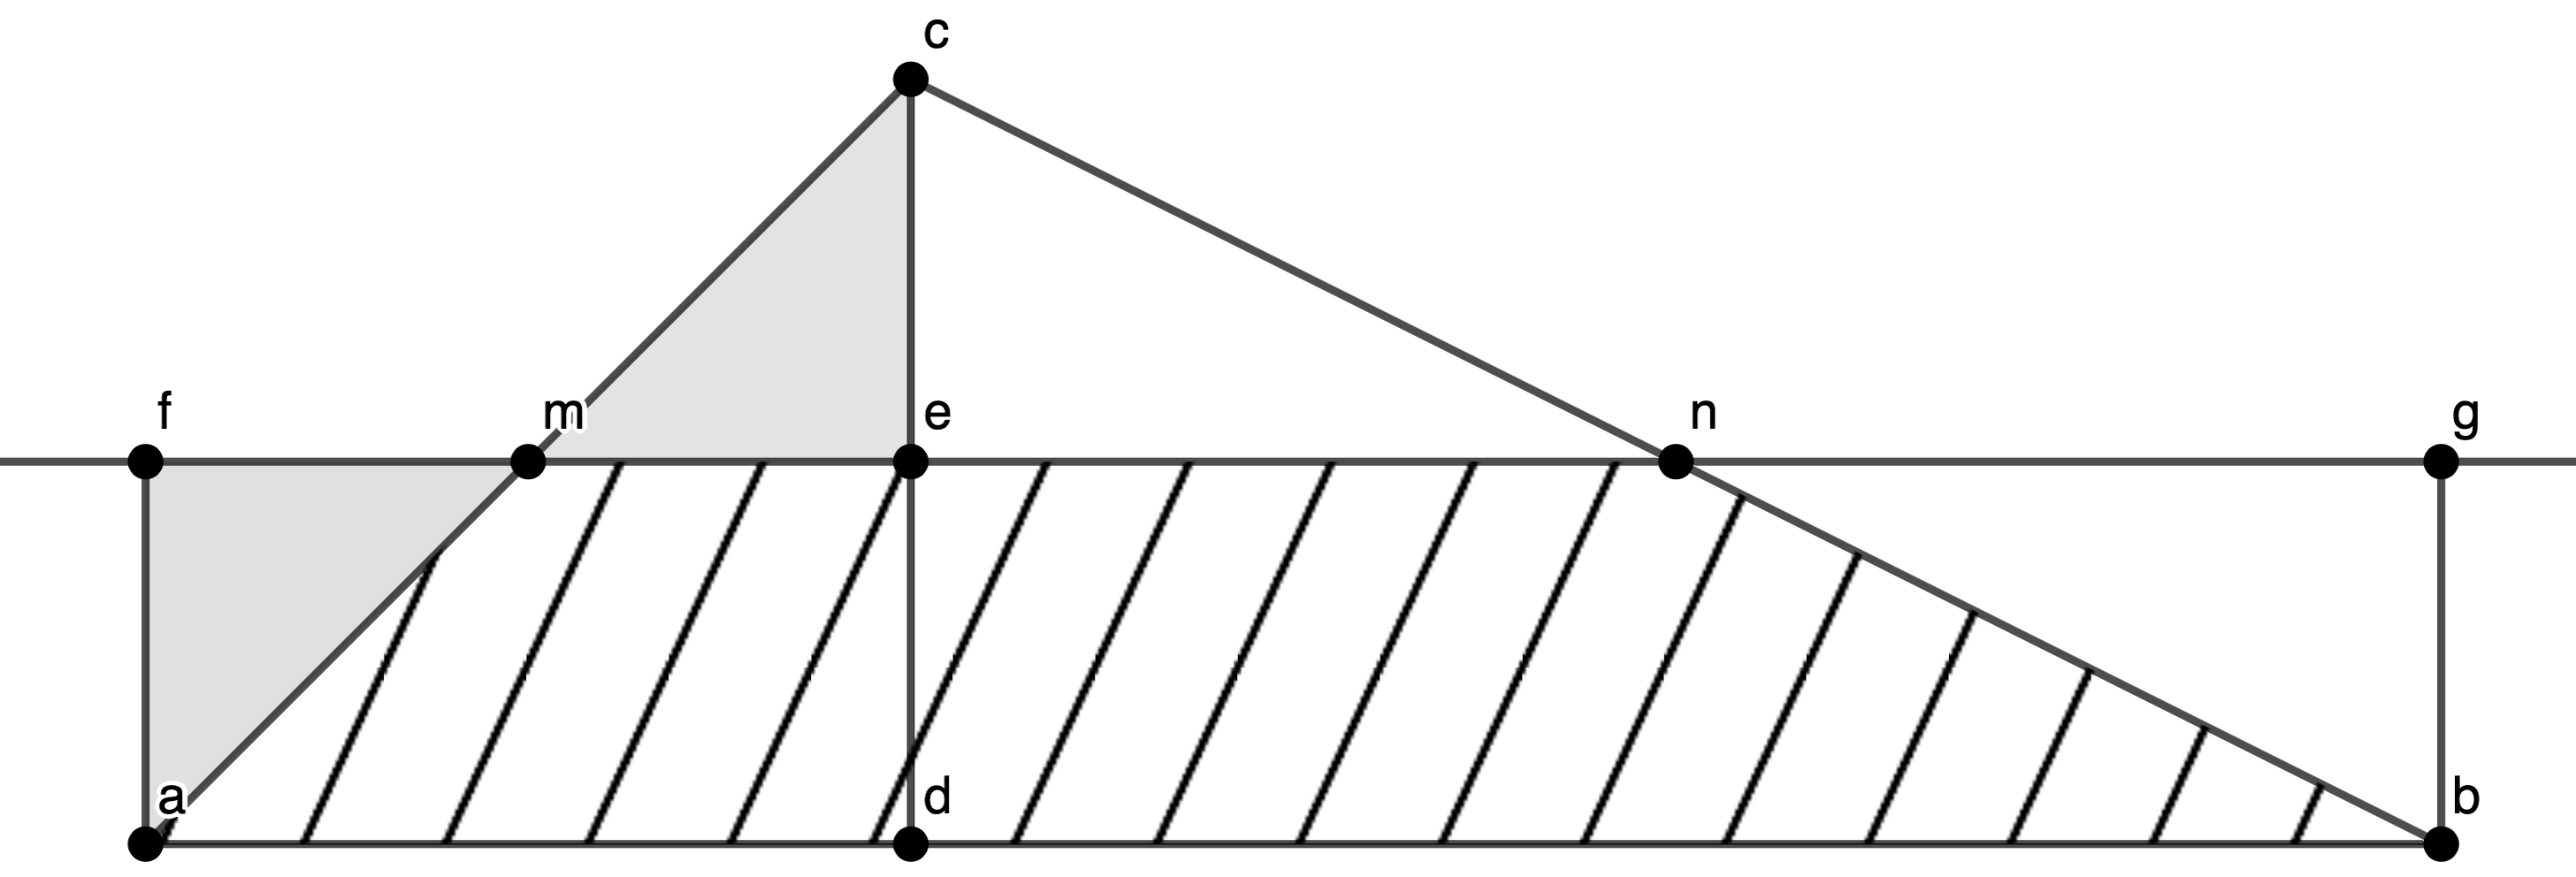
\includegraphics[scale=1.6]{DreieckLemma}
		\caption{Zerlegung eines Dreiecks in ein Rechteck}
		\label{Abb.1}
	\end{figure}
	
	\begin{lemma} \label{lemma:rechtecke}
		Zwei beliebige Rechtecke mit dem gleichen Flächeninhalt, sind zerlegungsgleich.
	\end{lemma}
	
	\begin{proof}
		Seien $P$ und $Q$ zwei Rechtecke mit dem gleichen Flächeninhalt, d. h. falls $h_P$ die Höhe und 
		$b_P$ die Breite des Rechtecks $P$ und $h_Q$ die Höhe und $b_Q$ die Breite des Rechtecks $Q$ sind, 
		dann soll gelten $h_P \cdot b_P = h_Q \cdot b_Q$ also auch
		\begin{align}
			\frac{b_P}{h_Q}=\frac{b_Q}{h_P}. \label{lemma:rechteck;1}
		\end{align}
		\begin{figure}[!htbp]
			\centering
			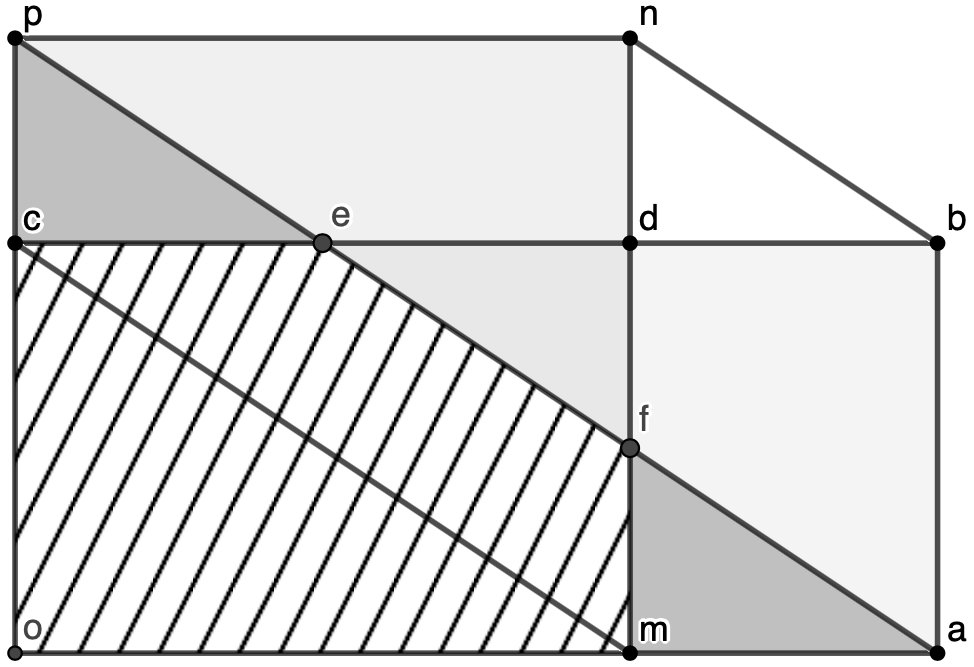
\includegraphics[scale=1.4]{Rechteck}
			\caption{Zerlegung zweier Rechtecke}
			\label{Abb.2}
		\end{figure}
		Seien $o,a,b,c$ die Eckpunkte des Dreiecks $P$ und $o,m,n,p$ die Eckpunkte des Dreiecks $Q$, siehe 
		Abbildung \ref{Abb.2}. 
		Wir verschieben hier $Q$ so auf auf $P$, dass beide eine gemeinsame Ecke $o$ mit rechtem Winkel haben. 
		Dies ändert nichts am Resultat. 
		Die Höhe $h_P$ soll also der Länge der Strecken $\overline{co}$ und $\overline{ab}$ entsprechen. Die 
		Breite $b_P$ soll der Länge der Strecken $\overline{oa}$ und $\overline{bc}$ entsprechen. Analog soll 
		$h_Q$ der Länge der Strecken $\overline{po}$ und $\overline{mn}$ und $b_Q$ der Länge der Strecken 
		$\overline{om}$ und $\overline{np}$ entsprechen. Wegen \ref{lemma:rechteck;1} sehen wir also, dass 
		die Strecken $\overline{mc}$ und $\overline{ap}$ parallel sind. Außerdem stellen wir fest, dass gilt
		\[ (b_P-b_Q)h_P=b_P h_P-b_Q h_P=h_Qb_Q-b_Qh_P=b_Q(h_Q-h_P) \]
		also auch
		\[\frac{b_P-b_Q}{h_Q-h_P}=\frac{b_Q}{h_P}. \]
		Damit folgt, dass die Dreiecke $oap$ und $dbn$ ähnlich sind und folglich sind die Strecken $\overline{ap}$ 
		und $\overline{nb}$ parallel. Hierbei sei $d$ der Schnittpunkt der Strecken $\overline{mn}$ und 
		$\overline{bc}$. Also sind die drei Strecken $\overline{mc}$, $\overline{ap}$ und $\overline{nb}$ 
		parallel. Nun unterscheiden wir zwei Fälle
		\begin{enumerate}
			\item \textsl{Fall:} Die Verbindungsstrecke $\overline{ap}$ der Eckpunkte schneidet das 
			Rechteck $omdc$ in den Punkten $e$, mit der Seite $\overline{dc}$ und $f$, mit der Seite $\overline{md}$ 
			, siehe Abbildung \ref{Abb.2}. Es gilt $2b_Q\geq b_P$.
			Also sind die beiden in der Abbildung grau hinterlegten Dreiecke $maf$ und $cep$ und die beiden 
			in der Abbildung hellgrau hinterlegten Dreiecke $abe$ und $fnp$ kongruent. Mit dem übrig gebliebenen 
			in der Abbildung schraffierten Fünfeck $omfec$ ist unsere Zerlegung komplett.
			
			\item \textsl{Fall:} Die Verbindungsstrecke $\overline{ap}$ der Eckpunkte schneidet das 
			Rechteck $omdc$ nicht, siehe Abbildung \ref{Abb.3}. 
			Es gilt also $2b_Q<b_P$. Sei nun $e$ hierbei der Mittelpunkt der Strecke $\overline{oa}$ und $k$ die 
			kleinste natürliche Zahl, wie oft man die Strecke $\overline{om}$ entlang der Strecke $\overline{oa}$ 
			legen muss, sd. wir einen Punkt $t$ erhalten der nicht mehr auf der Strecke $\overline{oe}$ liegt 
			sondern auf der Strecke $\overline{ea}$. Nun zerlegen wir das Rechteck $Q$ in $k$ Rechtecke, deren 
			Basis parallel ist zur Strecke $\overline{om}$, die wir nun entlang der neu enstandenen Strecke 
			$\overline{ot}$ legen. Wir erhalten, somit das zu $Q$ zerlegungsgleiche Rechteck $otuv$. 
			Sei die Breite dieses Rechtecks nun $b'$, die offensichtlich die Bedingung
			\[ 2b'>b_P \]
			erfüllt. Damit können wir nach dem ersten Fall sagen, dass die Rechtecke $P$ und $otuv$ 
			zerlegungsgleich sind. Nach Lemma \ref{lemma:transitiv} sind also auch $P$ und $Q$ zerlegungsgleich.
		\end{enumerate}
		Damit sind $P$ und $Q$ zerlegungsgleich.
	\end{proof}
	
	\begin{figure}[!htbp]
		\centering
		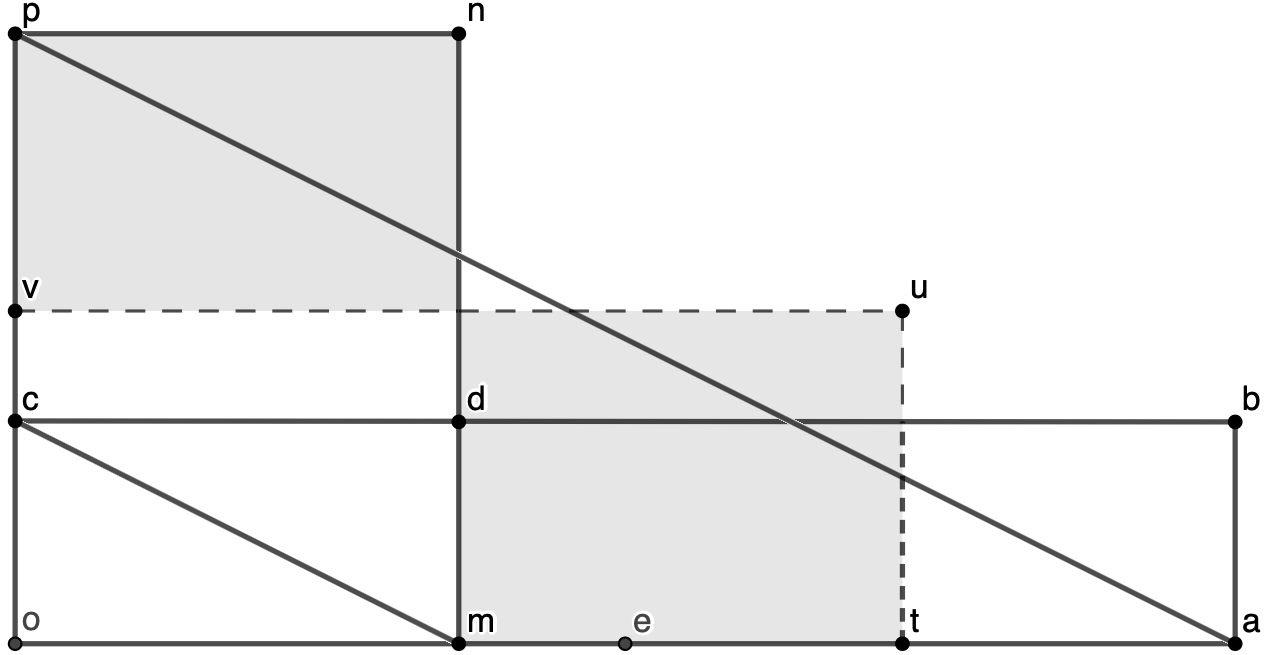
\includegraphics[scale=0.8]{Rechteck2}
		\caption{Zerlegung zweier Rechtecke}
		\label{Abb.3}
	\end{figure}
	
	\begin{theorem}[Bolyai-Gerwien Theorem] \label{theorem:bolyai-gerwien}
		Zwei beliebige Polygone mit dem gleichen Flächeninhalt sind zerlegungsgleich.
	\end{theorem}
	
	\begin{proof}
		Sei $P$ ein Polygon. Dann kann $P$ in endlich viele disjunkte Dreiecke zerlegt werden und jedes dieser 
		Dreiecke ist nach Lemma \ref{lemma:dreieck,rechteck} zerlegungsgleich zu einem Rechteck. Wir finden 
		also für $P$ die Darstellung
		\[ P\sim P_1+\ldots+P_n,\]
		wobei $P_1,\ldots,P_n$ Rechtecke sind. Nun nehmen wir eine beliebige Kante $\overline{a_0b_0}$ und 
		stellen die Lotgeraden auf den Eckpunkten $a_0$ und $b_0$ durch die Strecke $\overline{a_0b_0}$ 
		auf. Anschließend ziehen wir $n$ 
		parallele Strecken zu $\overline{a_0b_0}$, sd. der Flächeninhalt des Recheckts $a_{i-1}b_{i-1}b_ia_i$, 
		welches wir $R_i$ nennen, dem Flächeninhalt des Rechtecks $P_i$ entspricht, wobei $i=1,\ldots,n$. 
		Nach Lemma \ref{lemma:rechtecke} gilt also $P_i\sim R_i$ für alle $i$ und damit
		\[ P_1+\ldots+P_n\sim R_1+\ldots+R_n. \]
		Da $P\sim P_1+\ldots+P_n$ gilt also mit Lemma \ref{lemma:transitiv}
		\[ P\sim R_1+\ldots+R_n\]
		und damit zum Rechteck $a_0b_0b_na_n$. Damit ist jedes Polygon zerlegungsgleich zu einem Rechteck. \\
		Seien nun $P$ und $Q$ zwei Polygone mit gleichem Flächeninhalt, dann finden wir wie oben gezeigt 
		Rechtecke $R_1$ und $R_2$, sd.
		\[ P\sim R_1,\quad Q\sim R_2.\]
		Nach Lemma \ref{lemma:rechtecke} gilt also nun auch $R_1\sim R_2$ und damit folgt mit Lemma 
		\ref{lemma:transitiv} $P\sim Q$.
	\end{proof}
	
	Wir haben also nun gesehen, dass sich jedes beliebige Polygon in Dreiecke zerlegen lässt. Diese Dreiecke 
	sind nach Lemma \ref{lemma:dreieck,rechteck} zerlegungsgleich zu Rechtecken mit gleichem 
	Flächeninhalt. Zuletzt können wir mit Satz \ref{theorem:bolyai-gerwien} die Rechtecke zerlegen zu Rechtecken 
	mit gleicher Grundseite. Dieses Verfahren können wir nun auf beliebige Polygone mit gleichem Flächeninhalt 
	anwenden. Da diese Rechtecke nach Lemma \ref{lemma:rechtecke} zerlegungsgleich sind folgt mit der 
	Transitivität der Zerlegungsgleichheit aus Lemma \ref{lemma:transitiv} die Zerlegungsgleichheit der Polygone und 
	mit Proposition \ref{prop:zerl,erg} auch die Ergänzungsgleichheit. 
	Dies führt uns zu der Frage, ob das gleiche auch für dreidimensionale Polytope, also Polyeder, möglich ist.
	
	\textsl{Motivation:} Als Hilbert 1900 diese Frage auf dem internationalen Mathematikerkongress in Paris als 
	sein drittes von 23 Problemen stellte, vermutete er wohl schon, dass die Antwort 'Nein' ist. Im Folgenden wollen wir 
	uns zwei Beweise anschauen, die zeigen, dass es Polyeder gibt, die nicht zerlegungs- und ergänzungsgleich sind. 
	Der erste bezieht sich auf die Arbeit Max Dehn's, ein Schüler Hilberts, der ein Jahr später in seiner Habitilationsarbeit 
	die Aussage mithilfe der von ihm erfundenen Dehn-Invariante widerlegte. Der zweite Beweis...
	
	\section{Zerlegungsgleichheit von Polyedern; Dehn-Invariante}
	
	Im Folgenden setzen wir $d=3$ und betrachten Polyeder.
	
	Wir müssen uns zunächst überlegen, was mit den Kanten eines Polyeders $P$ passiert, wenn wir diesen in zwei 
	Polyeder $P_1$ und $P_2$ zerlegen. Sei $k$ also eine Kante des Polyeders $P$. Diese Kante hat die Länge 
	$\ell(k)=l$. Außerdem ist die Kante $k$ die Schnittmenge der zwei anliegenden Seitenflächen. Den Winkel zweier 
	solcher Flächen nennt man Diederwinkel. Sei also $w(k)=\varphi$ der zu $k$ gehörige Diederwinkel. Dann können 
	beim zerschneiden folgende Fälle eintreten
	\begin{enumerate}
		\item \label{bem:dehn;1} 
		Wir schneiden durch die Kante: Also enstehen zwei neue Kanten $k_1$ von $P_1$ und $k_2$ von $P_2$, 
		deren Kantenlängen sich zu der von $k$ addieren lassen und deren Winkel gleich dem von $k$ bleibt. 
		D. h. für $\ell(k_1)=l_1$ und $\ell(k_2)=l_2$ gilt $l=l_1 +l_2$.
		\item \label{bem:dehn;2} 
		Wir schneiden entlang der Kante: Also entstehen zwei neue Kanten $k_1$ von $P_1$ und $k_2$ von 
		$P_2$, deren Kantenlänge gleich der von $k$ ist und deren Winkel sich zu dem von $k$ addieren lassen. 
		D. h. für $w(k_1)=\varphi_1$ und $w(k_2)=\varphi_2$ gilt $\varphi=\varphi_1 +\varphi_2$.
		\item \label{bem:dehn;3} 
		Wir schneiden nicht durch die Kante: Die Kante $k$ lässt sich also entweder in $P_1$ oder $P_2$ 
		wiederfinden und sowohl Kantenlänge, als auch Diederwinkel bleiben gleich.
		\item \label{bem:dehn;4} 
		Bleibt nur noch der Sonderfall, wenn wir durch eine der Flächen von $P$ schneiden. Hierbei entstehen 
		aus dem nichts zwei neue Kanten $k_1$ von $P_1$ und $k_2$ von $P_2$, deren Länge der Länge des 
		Schnitts entsprechen und deren Winkel sich zu $\pi$ addieren lässt. D. h. für $w(k_1)=\varphi_1$ und 
		$w(k_2)=\varphi_2$ gilt $\varphi_1 +\varphi_2 =\pi$.
	\end{enumerate}
	Wir wollen also eine Operation, die in beiden Argumenten, sowohl in Länge als auch Diederwinkel, linear ist 
	und bei der wir einen Diederwinkel $\pi$ mit $0$ identifizieren. Dies führt uns auf das Tensorprodukt.
	
	\subsection{Tensoren}
	
	Wir kennen Tensoren bereits aus der linearen Algebra. Deshalb wiederholen wir noch einmal die universelle 
	Eigenschaft dieser.
	
	%\begin{proposition}[Universelle Eigenschaft]
	%	Sei $R$ ein kommutativer Ring mit Eins und seien $M$ und $N$ zwei $R$-Moduln. Dann gilt
	%	\begin{enumerate}
	%		\item Die Abbildung $\otimes: M\times N \to M\otimes_R N$ ist $R$-bilinear.
	%		\item Sei nun $L$ ein weiterer $R$-Modul und $\phi: M\times N \to L$ eine bilineare Abbildung. Dann 
	%		existiert genau eine lineare Abbildung $\eta: M\otimes_R N \to L$, sd. das folgende Diagramm 
	%		kommutiert:
	%		\begin{center}
	%			\begin{tikzpicture}
	%				\node(R1) at (0,0){$M\times N$};
	%				\node[right = 2 of R1](k){$L$};
	%				\node[below = 1 of R1](R2){$M\otimes N$};
	%				
	%				\draw[->] (R1) -- (k) node[midway,above]{$\phi$};
	%				\draw[->] (R1) -- (R2) node[midway,left]{$\otimes$};
	%				\draw[->,dashed] (R2) -- (k) node[midway,below]{$\exists ! \eta$};
	%			\end{tikzpicture}
	%		\end{center}
	%	\end{enumerate}
	%	Der $R$-Modul $M\otimes N$ ist bis auf Isomorphie eindeutig.
	%\end{proposition}
	
	\begin{proposition}[Universelle Eigenschaft] \label{prop:univeig}
		Sei $R$ ein kommutativer Ring mit Eins und seien $M$ und $N$ zwei $R$-Moduln. Dann ist das 
		\textsl{Tensorprodukt} $M\otimes_R N$ genau derjenige $R$-Modul zu dem es eine bilineare Abbildung 
		$\otimes: M\times N \to M\otimes_R N$ gibt, die die folgende universelle Eigenschaft erfüllt:
		\begin{center}
			Sei $L$ ein weiterer $R$-Modul und $\phi: M\times N \to L$ eine bilineare Abbildung. Dann 
			existiert genau eine lineare Abbildung $\eta: M\otimes_R N \to L$, sd. das folgende Diagramm 
			kommutiert:
			\begin{center}
				\begin{tikzpicture}
					\node(R1) at (0,0){$M\times N$};
					\node[right = 2 of R1](k){$L$};
					\node[below = 1 of R1](R2){$M\otimes N$};
					
					\draw[->] (R1) -- (k) node[midway,above]{$\phi$};
					\draw[->] (R1) -- (R2) node[midway,left]{$\otimes$};
					\draw[->,dashed] (R2) -- (k) node[midway,below]{$\exists ! \eta$};
				\end{tikzpicture}
			\end{center}
		\end{center}
		Gibt ein solches $R$-Modul $M\otimes_R N$, dann ist dieses bis auf Isomorphie eindeutig bestimmt.
	\end{proposition}
	
	\begin{proof}
		Für den Beweis sei auf Proposition 2.12 in Atiyah verwiesen.
	\end{proof}
	
	Also wissen wir nun, dass das Tensorprodukt folgende Eigenschaften erfüllt. Sei $R$ ein kommutitativer Ring 
	mit Eins und $R$-Moduln $M$ und $N$, dann gilt für alle $m,m'\in M$, $n,n'\in N$ und $r,r'\in R$
	\begin{align*}
		(mr+m'r'\otimes n)=(m\otimes n)\cdot r +(m'\otimes n)\cdot r' \\
		(m\otimes nr+n'r')=(m\otimes n)\cdot r+(m\otimes n')\cdot r'.
	\end{align*}
	
	Damit ist der bilineare Operator gefunden. Wir wollen für unser Problem den Spezialfall 
	$\setR \otimes_{\setZ} \setR / \pi\setZ$ betrachen. Hierbei identifizieren wir die Länge einer Kante mit dem 
	ersten Argument und tensorieren dies mit einem Winkel, wobei wir den Winkel $\pi$ mit 0 identifizieren.
	
	\subsection{Die Dehn-Invariante}
	
	\begin{definition}[Dehn-Invariante]
		Sei $P$ ein dreidimensionaler beschränkter Polyeder mit den Kanten $k_1,\ldots,k_n$. Dann definieren wir die 
		\textsl{Dehn-Invariante} $D(P)\in \setR \otimes_{\setZ}\setR/\pi \setZ$ durch
		\[ \sum_{i=1}^n \ell(k_i)\otimes [w(k_i)]. \]
	\end{definition}
	
	Wir müssen nun zeigen, dass die Dehn-Invariante sich beim Zerschneiden eines Polyeders sich nicht 
	verändert und somit eine Invariante ist.
	
	\begin{proposition}[Invarianz] \label{prop:invarianz}
		Sei $P$ ein Polyeder und $P=P_1+P_2$ eine Zerlegung von $P$ in zwei Polyeder $P_1$ und $P_2$, dann 
		gilt $D(P_1+P_2)=D(P_1)+D(P_2)$.	
	\end{proposition}
	
	\begin{proof}
		Sei $P$ ein beschränkter Polyeder, den wir in zwei Polyeder $P_1$ und $P_2$ zerschneiden. 
		Die Summe der  Dehn-Invarianten der einzelnen Polyeder soll also gerade der Dehn-Invariante von $P$ 
		entsprechen. Dazu betrachten wir die Kanten der Polyeder und überlegen was für die Summanden gilt. Es 
		reicht die Fälle zu betrachten, die wir am Anfang des Kapitels erwähnt haben.
		\begin{itemize}
			\item Zu \ref{bem:dehn;1}: Beim schneiden durch eine Kante $k$ von $P$ entstehen zwei 
			neue Kanten $k_1$ von $P_1$ und $k_2$ von $P_2$, wobei die Längen sich addieren und der Winkel 
			gleich bleibt. Es gilt
			\[ \ell(k_1)\otimes_{\setZ}w(k) + \ell(k_2)\otimes_{\setZ}w(k)=(\ell(k_1)+\ell(k_2))\otimes_{\setZ}w(k)=
			\ell(k)\otimes_{\setZ}w(k).\]
			Also verändert sich die Dehn-Invariante nicht.
			\item Zu \ref{bem:dehn;2}: Beim schneiden entlang einer Kante $k$ von $P$ entstehen zwei neue Kanten 
			$k_1$ von $P_1$ und $k_2$ von $P_2$, wobei die Längen gleich bleiben und die Winkel sich addieren. 
			Es gilt
			\[ \ell(k)\otimes_{\setZ} w(k_1)+\ell(k)\otimes_{\setZ}w(k_2)=\ell(k)\otimes_{\setZ}(w(k_1)+w(k_2))=
			\ell(k)\otimes_{\setZ}w(k). \]
			Also verändert sich auch hier die Dehn-Invariante nicht.
			\item Zu \ref{bem:dehn;3}: Wir schneiden nicht durch die Kante $k$ von $P$, also ändert sich auch der 
			Summand nicht und damit die Dehn-Invariante.
			\item Zu \ref{bem:dehn;4}: Beim Schneiden durch eine Fläche entstehen zwei neue Kanten $k_1$ von 
			$P_1$ und $k_2$ von $P_2$, deren Länge gleich ist und Winkel sich zu $\pi$ addieren lässt. Es gilt 
			\[ \ell(k_1)\otimes_{\setZ}w(k_1)+\ell(k_1)\otimes_{\setZ}w(k_2)=\ell(k_1)\otimes_{\setZ}(w(k_1)+w(k_2))=
			\ell(k_1)\otimes_{\setZ}\pi=\ell(k_1)\otimes_{\setZ}0=0. \]
			Also ändert auch dies nichts an der Dehn-Invariante.
		\end{itemize}
		Im Beweis haben wir lediglich die Bilinearität des Tensorprodukts ausgenutzt.		
	\end{proof}
	
	\begin{proposition} \label{prop:cong,dehn}
		Seien $P$ und $Q$ zwei Polyeder, sd. $P\cong Q$, dann gilt $D(P)=D(Q)$.
	\end{proposition}
	
	\begin{proof}
		Isometrien erhalten sowohl Kantenlängen, als auch Diederwinkel der Polyeder und damit bleibt auch 
		die Dehn-Invariante unverändert.
	\end{proof}
	
	\begin{theorem}[Dehn] \label{thm:dehn}
		Seien $P$ und $Q$ zerlegungsgleiche Polyeder, dann gilt $D(P)=D(Q)$ und $vol(P)=vol(Q)$.
	\end{theorem}
	
	\begin{proof}
		Seien $P=P_1+\ldots+P_n$ und $Q=Q_1+\ldots+Q_n$ die Zerlegungen von $P$ und 
		$Q$, also $P_i\cong Q_i$ für alle $i=1,\ldots,n$. Dann folgt mit Proposition \ref{prop:zerl,vol}
		dass $vol(P)=vol(Q)$. Außerdem gilt mit Proposition \ref{prop:cong,dehn}
		und mit Proposition \ref{prop:invarianz}
		\[D(P)=D(P_1+\ldots+P_n)=\sum_{i=1}^n D(P_i) =\sum_{i=1}^n D(Q_i)=D(Q_1+\ldots+Q_n)=D(Q).\]
	\end{proof}
	
	Wir wollen uns nun zur Berechnung der Dehn-Invariante einiger Polyeder ein paar Eigenschaften des Tensorprodukts $\setR\otimes_{\setZ}\setR /\pi\setZ$ anschauen. Dazu wollen wir zeigen, dass unser Tensorprodukt isomorph zum Tensorprodukt  
	$\setR\otimes_{\setQ}\setR /\pi\setQ$ ist, hierzu benötigen wir ein 
	paar Resultate 
	aus der Kommutativen Algebra. \\
	Sei nun $R$ ein Integritätsring, wir wollen nun 
	Brüche einführen. Sei dazu $S$ eine multiplikative Teilmenge von $R$, das heißt  
	$1\in S$ und $S$ ist unter Multiplikation abgeschlossen, also ein Monoid. Wir 
	definieren die Relation $\equiv$ auf $R\times S$ durch
	\[(r_1,s_1)\equiv(r_2,s_2)\quad \Leftrightarrow\quad r_1 s_2 =r_2 s_1\]
	für Elemente $r_1,r_2\in R$ und $s_1,s_2\in S$. \\
	Wir stellen fest, dass diese Relation  eine Äquivalenzrelation ist. Die 
	Reflexivität und Symmetrie ist klar, wir zeigen also noch die Transitivität.
	Es gelte also $(r_1,s_1)\equiv(r_2,s_2)$ und $(r_2,s_2)\equiv(r_3,s_3)$ für 
	$r_1,r_2,r_3\in R$ und $s_1,s_2,s_3\in S$, also gilt $r_1 s_2= r_2 s_1$ und 
	$r_2 s_3 =r_3 s_2$ und damit $r_1 s_2 r_2 s_3 =r_2 s_1 r_3 s_2$. Falls $r_2=0$ 
	ist klar, dass $(r_1,s_1)\equiv(r_3,s_3)$ gilt, falls $r_2\neq 0$ können wir $r_2$ aus der Gleichung streichen und es folgt 
	$r_1 s_3=r_3 s_1$ und damit $(r_1,s_1)\equiv(r_3,s_3)$. \\
	Wir schreiben $\frac{r}{s}$ für die Äquivalenzklasse von $(r,s)$ und $S^{-1}R$ 
	für die Menge aller Äquivalenzklassen. Wir können $S^{-1}R$ nun eine Ringstruktur geben, indem wir die Addition und Multiplikation wie folgt definieren
	\begin{align*}
		\left(\frac{r_1}{s_1}\right)+\left(\frac{r_2}{s_2}\right)
		&=\left(\frac{r_1s_2+r_2s_1}{s_1s_2}\right) \\
		\left(\frac{r_1}{s_2}\right)\cdot\left(\frac{r_2}{s_2}\right)
		&=\left(\frac{r_1r_2}{s_1s_2}\right)
	\end{align*}
	für alle $r_1,r_2\in R$ und $s_1,s_2\in S$. Wir stellen fest, dass 
	$S^{-1}R$ sogar ein kommutativer Ring mit Eins ist. Außerdem ist 
	$S^{-1}R$ gerade der Quotientenkörper von $R$, falls $S=R\setminus\{0\}$ ist. Betrachten wir also beispielweise den Ring 
	$\setZ$ mit der multiplikativen Teilmenge $S=\setZ\setminus\{0\}$, so 
	ist $S^{-1}\setZ$ gerade der Quotientenkörper von $\setZ$, also 
	$\setQ$. Wir können diese Konstruktion nun auch auf Moduln fortführen. 
	Haben wir ein $R$-Modul $M$, dann definieren wir 
	die Äquivalenzrelation wie oben, nur auf $M$, und erhalten die 
	Äquivalenzklassen $\frac{m}{s}$ für Elemente $m\in M$ und $s\in S$. 
	Dann ist $S^{-1}M$ gerade die Menge solcher Brüche und wir erhalten 
	mit $S^{-1}M$ ein $S^{-1}R$-Modul mit der natürlichen Definition 
	der Addition und skalaren Multiplikation. Haben wir nun einen 
	$R$-Modulhomomorphismus $f:M\to N$, dann führt uns dies zu einem 
	$S^{-1}R$-Modulhomomorphismus $S^{-1}f:S^{-1}M\to S^{-1}N$, indem $S^{-1}f$ 
	Elemente $\frac{m}{s}$ auf $\frac{f(m)}{s}$ abbildet. Damit gilt also 
	\[S^{-1}(f\circ g)=(S^{-1}f)\circ(S^{-1}g),\]
	für Modulhomomorphismen $f$ und $g$.
	
	\begin{lemma} \label{lemma:Buch;exakt}
		Sei $R$ ein Integritätsring und $M,M_1,M_2$ seien $R$-Moduln. Weiter 
		sei die Sequenz
		\begin{align}
			M_1\xrightarrow{f}M\xrightarrow{g}M_2 \label{lemma:exakt;1}
		\end{align}
		exakt in $M$. Dann ist die Sequenz
		\[S^{-1}M_1 \xrightarrow{S^{-1}f}S^{-1}M\xrightarrow{S^{-1}g}S^{-1}M_2\]
		exakt in $S^{-1}M$.
	\end{lemma}
	
	Siehe dazu auch \cite[Proposition 3.3]{introductiontocomalg}.
	
	\begin{proof}
		Sei $m_1\in M_1$ dann gilt $f(m_1)\in im(f)=ker(g)$, wegen der Exaktheit 
		von \ref{lemma:exakt;1} in $M$ und damit ist $f(m_1)=0$. Also gilt 
		$f\circ g=0$ und weiterhin
		\[S^{-1}f \circ S^{-1}g = S^{-1}(f\circ g)=S^{-1}(0)=0.\]
		Wir erhalten also
		\[im(S^{-1}f)\subset ker(S^{-1}g).\]
		Um die umgekehrte Inklusion zu zeigen wählen wir 
		$\frac{m}{s}\in ker(S^{-1}g)$, das heißt $\frac{g(m)}{s}=0$ in $S^{-1}M_2$. 
		Das wiederum bedeutet, dass $g(m)=0$ in $M_2$, da $R$ ein Integritätsring 
		ist, also auch $m\in ker(g)=im(f)$, wegen der Exaktheit von $M$ in 
		\ref{lemma:exakt;1}. Also gibt es ein $m_1\in M_1$ mit $f(m_1)=m$ und damit 
		gilt
		\[\frac{m}{s}=\frac{f(m_1)}{s}=(S^{-1}f)\left(\frac{m_1}{s}\right)\in im(S^{-1}f).\]
		Es folgt 
		\[ker(S^{-1}g)\subset im(S^{-1}f).\]
	\end{proof}

	Nun zurück zu unserem Problem. Wir wollen nun wissen, was passiert wenn 
	wir in dem $\setZ$-Modul $\setR /\pi\setZ$ Brüche einführen. Um das 
	zu verstehen, hilft uns das folgende Resultat.
	
	\begin{lemma}
		Sei $R$ ein Integritätsring, $M$ ein $R$-Modul und 
		$N$ ein $R$-Untermodul von $M$. Weiter sei $S$ eine multiplikative 
		Teilmenge von $R$, dann sind die $S^{-1}R$-Moduln $S^{-1}(M/N)$ und 
		$S^{-1}M/S^{-1}N$ isomorph.
	\end{lemma}
	
	Siehe \cite[Korollar 3.4 (iii)]{introductiontocomalg}.
	
	\begin{proof}
		Wir betrachten hierzu die Sequenz
		\[0\to N\xrightarrow{f} M\xrightarrow{g} M/N\xrightarrow{h} 0,\]
		wobei $f,g$ und $h$ hier Modulhomomorphismen sind. Die Funktion 
		$f$ bettet das Untermodul $N$ in $M$ ein, also gilt 
		$im(f)=N$. Weiter bildet die Funktion $g$ gerade die Elemente aus $M$ 
		auf deren Äquivalenzklassen in $M/N$ ab und da für alle $n\in N\subset M$ 
		gilt, dass $g(n)=[n]=0$ in $M/N$, folgt auch, dass $ker(g)=N$. Damit 
		ist die Sequenz in $M$ exakt. \\
		Weiter ist $im(g)=M/N$ und da $h$ die Nullabbildung ist, gilt $ker(h)=M/N$. 
		Also ist die Sequenz auch in $M/N$ exakt. \\
		Wir wenden nun $S^{-1}$ auf die exakte Sequenz an, dann ist die Sequenz
		\begin{align}
			0\to S^{-1}N \xrightarrow{S^{-1}f} S^{-1}M \xrightarrow{S^{-1}g}
			S^{-1}(M/N)\to 0 \label{lemma:Brüche;1}
		\end{align}
		mit Lemma \ref{lemma:Buch;exakt} exakt. \\
		Wir wollen nun den Homomorphiesatz auf den Modulhomomorphismus 
		$S^{-1}g$ anwenden und erhalten mit der Exaktheit von \ref{lemma:Brüche;1} 
		in $S^{-1}M$
		\[ S^{-1}(M/N)=im(S^{-1}g)\simeq S^{-1}M/ker(S^{-1}g) =S^{-1}M/im(S^{-1}f)=S^{-1}M/S^{-1}N.\]
	\end{proof}
	
	Wenden wir das nun auf das $\setZ$-Modul $\setR /\pi\setZ$ mit 
	$S=\setZ\setminus\{0\}$ an, dann sind die $(\setZ\setminus\{0\})^{-1}\setZ$- also $\setQ$-Moduln 
	$(\setZ\setminus\{0\})^{-1}(\setR /\pi\setZ)$ und 
	$\left((\setZ\setminus\{0\})^{-1}\setR\right) /\left((\setZ\setminus\{0\})^{-1}\pi\setZ\right)$ 
	isomorph. Wir bemerken, dass $(\setZ\setminus\{0\})^{-1}\setR\simeq\setR$ und 
	$(\setZ\setminus\{0\})^{-1}\pi\setZ\simeq\pi\setQ$. Damit gilt also 
	\[ (\setZ\setminus\{0\})^{-1}(\setR /\pi\setZ)\cong \setR/\pi\setQ.\]
	
	\begin{lemma} \label{lemma:lociso}
		Sei $R$ ein Integritätsring und $M$ ein $R$-Modul. Dann gibt es einen 
		eindeutigen Isomorphismus
		\[f:S^{-1}R\otimes_R M\to S^{-1}M\]
		zwischen den $S^{-1}R$-Moduln, sd.
		\begin{align}
			f\left(\frac{r}{s}\otimes m\right)=\frac{rm}{s} \label{lemma:lociso;1}
		\end{align}
		für alle $r\in R$, $m\in M$ und $s\in S$.
	\end{lemma}
	
	Der Beweis richtet sich nach \cite[Proposition 3.5]{introductiontocomalg}.
	
	\begin{proof}
		Die Abbildung $g:S^{-1}R\times M\to S^{-1}M$ mit $g\left(\frac{r}{s},m\right)=\frac{rm}{s}$ ist bilinear, da 
		\begin{align*}
			&g\left(\lambda_1\left(\frac{r_1}{s_1}+\frac{r_2}{s_2}\right),
			\lambda_2 (m_1+m_2)\right)=g\left(\frac{\lambda_1 (r_1 s_2+r_2
			 s_1)}{s_1s_2},\lambda_2(m_1+m_2)\right) \\
			&=\frac{\lambda_1(r_1s_2+r_2s_1)\lambda_2(m_1+m_2)}{s_1s_2}\\
			&=\lambda_1\lambda_2\left(\frac{r_1(m_1+m_2)}{s_1}+
			\frac{r_2(m_1+m_2)}{s_2}\right) \\
			&=\lambda_1\lambda_2 \left(g\left(\frac{r_1}{s_1},m_1\right)
			+g\left(\frac{r_1}{s_1},m_2\right)+g\left(\frac{r_2}{s_2},m_1\right)+
			g\left(\frac{r_2}{s_2},m_1\right)\right)
		\end{align*}
		für alle $r_1,r_2,\lambda_1,\lambda_2\in R$, $s_1,s_2 \in S$ und 
		$m_1,m_2\in M$ gilt. Damit gibt es mit der universellen Eigenschaft 
		des Tensorprodukts (Proposition \ref{prop:univeig}) einen 
		$R$-Modulhomomorphismus $f:S^{-1}R\otimes_R M\to S^{-1}M$, sd. 
		\ref{lemma:lociso;1} gilt. Es ist klar, dass $f$ surjektiv ist, 
		dazu wählen wir $r=1$ und erhalten somit alle Elemente aus 
		$S^{-1}M$. Weiter ist $f$ auch eindeutig bestimmt durch 
		\ref{lemma:lociso;1}. \\
		Wir zeigen also noch die Injektivität. Dazu betrachten wir die 
		Elemente von $S^{-1}R\otimes_R M$. Sei also 
		\[\sum_{i=1}^n \frac{r_i}{s_i}\otimes m_i \in S^{-1}R\otimes_R M\]
		ein beliebiges Element, dann definieren wir
		\[s:=\prod_{i=1}^n s_i\in S,\qquad t_i:=\prod_{\genfrac{}{}{0pt}{1}{j=1}{j\neq i}}^n s_j\in S\]
		und es gilt 
		\[\sum_{i=1}^n \frac{r_i}{s_i}\otimes m_i =
		\sum_{i=1}^n \frac{r_it_i}{s}\otimes m_i =\sum_{i=1}^n 
		\frac{1}{s}\otimes r_i t_i m_i =\frac{1}{s}\otimes\sum_{i=1}^n
		\underbrace{r_it_im_i}_{\in M}.\]
		Wir können also jedes Element aus $S^{-1}R\otimes_R M$ in der Form 
		\[\frac{1}{s}\otimes m\]
		schreiben. Betrachten wir nun den Kern von $f$. Sei also 
		$\frac{1}{s}\otimes \in ker(f)\subset S^{-1}R\otimes_R M$, dh. 
		$f\left(\frac{1}{s}\otimes m\right)=0$. Da $R$ ein 
		Integritätsring ist folgt also mit $f\left(\frac{1}{s}\otimes m\right)=\frac{m}{s}=0$, dass $m=0$ und damit gilt
		\[\frac{1}{s}\otimes m =\frac{1}{s}\otimes 0=0.\]
		Damit ist $f$ bijektiv, also der gesuchte Isomorphismus.
	\end{proof}
	
	Es lässt sich nun folgendes Resultat zeigen, siehe dazu auch \cite{introductiontocomalg}[Proposition 3.7].
	
	\begin{proposition}\label{prop:tensoriso}
		Seien $M$ und $N$ zwei $R$-Moduln, dann gibt es einen eindeutigen 
		Isomorphismus 
		\[f:S^{-1}M\otimes_{S^{-1}R}S^{-1}N\to S^{-1}(M\otimes_R N)\]
		zwischen den $S^{-1}R$-Moduln, sd.
		\[f\left(\frac{m}{s_1}\otimes\frac{n}{s_2}\right)=\frac{m\otimes n}{s_1s_2}.\]
	\end{proposition}

	\begin{proof}
		Es gilt mit Lemma \ref{lemma:lociso} und den kanonischen Isomorphismen des 
		Tensorprodukts
		\begin{align*}
			S^{-1}M\otimes_{S^{-1}R}S^{-1}N &\overset{\ref{lemma:lociso}}{\simeq}
			(S^{-1}R\otimes_R M)\otimes_{S^{-1}R}(S^{-1}R\otimes_R N) \\
			&= M\otimes_R (\underbrace{S^{-1}R\otimes_{S^{-1}R S^{-1}R}}_{\simeq S^{-1}R})\otimes_R N \\
			&\simeq M\otimes_R S^{-1}R \otimes_R N \\
			&= S^{-1}R \otimes_R(M\otimes_R N) \\
			&\overset{\ref{lemma:lociso}}{\simeq} S^{-1}(M\otimes_R N).
		\end{align*}
	\end{proof}
	
	Dies lässt sich nun auf unser Tensorprodukt 
	$\setR\otimes_{\setZ}\setR /\pi\setZ$ anwenden, indem wir $R=\setZ$, $M=\setR$ und $N=\setR /\pi\setZ$ setzen und mit 
	$S=\setZ\setminus\{0\}$ und dem obigen Resultat ergibt sich 
	dann
	\begin{align*}
		S^{-1}R\simeq\setQ,\qquad S^{-1}M\simeq\setR
		\quad\text{ und }\quad S^{-1}N\simeq\setR /\pi\setQ.
	\end{align*}
	Weiterhin gilt
	\[S^{-1}(M\otimes_R N)\simeq \setR\otimes_\setZ\setR/\pi\setZ,\]
	denn mit der Bilinearität des Tensorprodukt gilt für 
	\begin{align*}
		(\setZ\setminus\{0\})^{-1}(\setR /\pi\setZ)&\simeq
		\left.\left\langle \left\{\frac{r\otimes s}{z}\right\vert
		 r\in\setR,s\in\setR/\pi\setZ,s\in\setZ\setminus\{0\}\right\}\right\rangle \\
		 &\simeq \left.\left\langle \left\{\frac{r}{z}\otimes s\right\vert r\in\setR,s\in\setR/\pi\setZ,s\in\setZ\setminus\{0\}\right\}
		 \right\rangle \\
		 &\simeq (\setZ\setminus\{0\})^{-1}\setR\ \ \otimes_\setZ\  \setR/\pi\setZ \\
		 &\simeq \setR\otimes_\setZ \setR/\pi\setZ,
	\end{align*}
	wobei wir mit $\langle\ \cdot\ \rangle$ hier das Erzeugnis meinen.
	Insgesamt erhalten wir also mit der Proposition
	\begin{align}
		\setR\otimes_\setZ\setR/\pi\setZ\simeq\setR\otimes_\setQ\setR/\pi\setQ. \label{tensor=0}
	\end{align}
	Wir können die Dehn-Invariante also auch auf dem $\setQ$-Vektorraum 
	$\setR\otimes_\setQ\setR/\pi\setQ$ betrachten, was uns zu der folgenden 
	Tatsache führt.
	
	\begin{theorem} \label{bem:dehn=0}
		Seien $x\in \setR$ und $y\in\setR/\pi\setQ$ Elemente, dann gilt
		\[ x\otimes y =0 \quad \Leftrightarrow \quad x=0 \ \lor\ y\in\pi\setQ.\]
	\end{theorem}
	
	\begin{proof}
		Die Rückrichtung ist schnell gezeigt, 
		denn für $x\in\setR$ mit $x\neq 0$ und $y=\pi\frac{p}{q}\in\setQ$, wobei $p\in\setZ$ und $q\in\setN$, gilt
		\[ x\otimes y =x\otimes\pi \frac{p}{q} =xp\otimes\frac{\pi}{q} =q\frac{xp}{q}
		\otimes\frac{\pi}{q} = \frac{xp}{q}\otimes\pi =\frac{xp}{q}\otimes 0=0.\]
		Dabei haben wir $p$ zuerst nach links und danach $q$ nach rechts bewegt. \\
		Zur Hinrichtung: Betrachte $\pi\setQ$ ist $1$-dimensionaler $\setQ$-
		Vektorraum mit Basis $\{\pi\}$ und $\pi\setQ\subset\setR$ ist 
		Untervektorraum von $\setR$ als $\setQ$-Vektorraum. Wir können also nun 
		unsere Basis mit dem Lemma von Zorn auf ganz $\setR$ fortsetzen. 
		Also hat $\setR$ als $\setQ$-Vektorraum die Basis
		\[\{\pi\}\dot\bigcup B,\]
		wobei $B$ die Menge ist mit der wir $\{\pi\}$ zu einer Basis von $\setR$ 
		ergänzen. Weiterhin gilt auch
		\begin{align*}
			\setR&\simeq\pi\setQ\oplus\bigoplus_{b\in B}b\setQ\qquad\text{und}\\
			\setR /\pi\setQ&\simeq\qquad\ \ \bigoplus_{b\in B}b\setQ.
		\end{align*}
		Damit ist
		\[\left\{(b_1\otimes b_2)\left\vert b_1\in\pi\setQ\oplus\bigoplus_{b\in B}b\setQ,\ b_2\in \bigoplus_{b\in B}b\setQ\right\}\right.\]
		eine Basis von $\setR\otimes_\setQ\setR/\pi\setQ$. \\
		Zwei Elemente $x\in\setR$ und $y\in\setR/\pi\setQ$ haben also die 
		Darstellung
		\begin{align*}
			x&=\alpha\pi+\sum_{b\in B}\beta_b b \\
			y&= \qquad\ \sum_{b'\in B}\gamma_{b'}b,
		\end{align*}
		wobei $\alpha,\beta_b,\gamma_{b'}\in\setQ$ für alle $b,b'\in B$ sind. 
		Falls nun $x\otimes y=0$ gilt also
		\[0=x\otimes y=\left(\alpha\pi+\sum_{b\in B}\beta_b b\right)\otimes
		\left(\sum_{b'\in B}\gamma_{b'}b\right)=\sum_{b'\in 
		B}\alpha\gamma_{b'}(\pi\otimes b')+\sum_{\genfrac{}{}{0pt}{1}{b\in B}
		{b'\in B}} \beta_b\gamma_{b'}(b\otimes b').\]
		Da $(\pi\otimes b')$ und $(b\otimes b')$ linear unabhängig sind für alle  
		$b,b'\in B$ folgt
		\[\alpha\gamma_{b'}=0\qquad\text{und}\qquad \beta_b\gamma_{b'}=0\]
		für alle $b,b'\in B$. 
		\begin{enumerate}
			\item Falls $\alpha\neq 0$, dann sind $\gamma_{b'}=0$ für alle 
			$b'\in B$ und damit ist $y=0$, also $y\in \pi\setQ$.
			\item Falls $\alpha=0$, dann sind die $\gamma_{b'}$ beliebig. 
			Angenommen es gibt also ein $b\in B$, sd. $\beta_b \neq 0$, dann 
			muss $\gamma_{b'}=0$ für alle $b'\in B$ damit $\beta_b\gamma_{b'}=0$ 
			für alle $b'\in B$ gilt. Das wiederum bedeutet $y=0$ und wir sind hier 
			fertig. Falls also $\beta_b=0$ für alle $b\in B$, folgt mit $\alpha=0$, 
			dass $x=0$.
		\end{enumerate}
		Damit haben wir die Aussage gezeigt.
	\end{proof}

	Wir bemerken, dass wir für die Hinrichtung also das Auswahl-Axiom 
	benutzt haben. Jedoch ist klar, dass wir bei einer konkreten Berechnung der 
	Dehn-Invariante nur endlich viele Polyeder haben, diese somit auch 
	nur einen endlich-dimensionalen $\setQ$-Untervektorraum von $\setR$ aufspannen und wir somit nicht auf das Auswahl-Axiom angewiesen sind. Wir 
	werden später sehen, dass wir im Beweis der Bricardschen Bedingung 
	vollkommen auf dieses verzichten können.
	
	Wir erhalten also auch:
	
	\begin{corollary}
		Seien $x\in\setR$ und $y\in\setR/\pi\setQ$ Elemente, dann gilt
		\[ x\otimes y\neq0\quad\Leftrightarrow\quad x\neq 0 \ \land\ y\notin\pi\setQ. \]
	\end{corollary}
	
	Folglich ist die Dehn-Invariante eines Polyeders $0$, falls dessen Diederwinkel alle in $\pi\setQ$ liegen. \\
	
	Wir können nun die Dehn-Invarianten einiger Polyeder berechnen.
	
	\begin{example}[Quader] \label{exp:quader}
		Sei $P$ ein dreidimensionaler Quader. Dann gilt für alle Kanten $k$ von $P$, dass $w(k)=\frac{\pi}{2}$. 
		Also gilt $w(k)\in \pi\setQ$ für alle Kanten $k$ und nach Bemerkung \ref{bem:dehn=0} folgt
		\[ D(P)=0. \]
	\end{example}
	
	\begin{example}[regulärer Tetraeder] \label{exp:regTetr}
		Sei $P$ ein dreidimensionaler regulärer Tetraeder, also haben alle Kanten von $P$ die gleiche Länge $l$ und 
		den gleichen Diederwinkel $\alpha$. Seien $A,B,C,D$ die Ecken von $P$ wie in Abbildung \ref{Abb.4}. 
		Sei $F$ der Mittelpunkt der Strecke $\overline{BC}$, also $|BF|=\frac{l}{2}$ und damit ist nach Pythagoras 
		$|AF|=\frac{\sqrt{3}}{2}l=|DF|$. Der Mittelpunkt $E$ des Dreiecks $ABC$ hat gerade den Abstand 
		$\frac{\sqrt{3}}{3 \cdot 2}l=\frac{l}{2\sqrt{3}}$ zu $F$ und schließlich gilt mit Pythagoras
		\[\cos(\alpha)=\frac{\frac{l}{2\sqrt{3}}}{\frac{\sqrt{3}}{2}l}=\frac{1}{3}\quad\text{also}
		\quad \alpha=\arccos\left(\frac{1}{3}\right). \]
		Damit können wir die Dehn-Invariante berechnen. Es gibt sechs Kanten der Länge $l$, die alle den 
		Diederwinkel $\arccos\left(\frac{1}{3}\right)$ haben, also
		\[ D(P)=\sum_{i=1}^6 l\otimes_{\setZ}\arccos\left(\frac{1}{3}\right)=6l\otimes_{\setZ}\arccos\left(\frac{1}{3}\right).\]
	\end{example}
	
	\begin{figure}[!htbp]
		\centering
		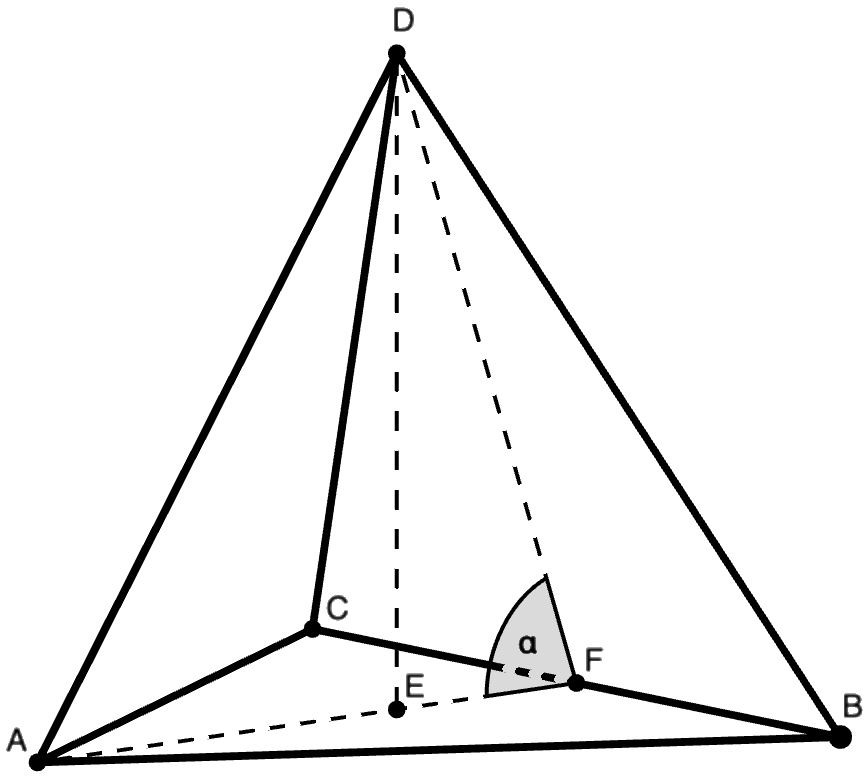
\includegraphics[scale=0.2]{RegulTetraeder}
		\caption{Ein regulärer Tetraeder}
		\label{Abb.4}
	\end{figure}
	
	\begin{proposition} \label{prop:irr}
		Für alle ungeraden $n\in\setN$ mit $n\geq 3$ gilt, $\frac{1}{\pi}\arccos\left(\frac{1}{\sqrt{n}}\right)$ ist irrational.
	\end{proposition}
	
	\begin{proof}
		Zuerst stellen wir fest, dass mit dem Additionstheorem
		\[\cos(\alpha)+\cos(\beta)=2\cos\left(\frac{\alpha+\beta}{2}\right)\cos\left(\frac{\alpha-\beta}{2}\right) \]
		für $\alpha=(k+1)\varphi$ und $\beta=(k-1)\varphi$ gilt
		\begin{align*}
			\cos\left((k+1)\varphi\right)+\cos\left((k-1)\varphi\right)=&2\cos\left(\frac{(k+1)\varphi+(k-1)\varphi}{2}\right)
			\cos\left(\frac{(k+1)\varphi-(k-1)\varphi}{2}\right) \\
			=& 2\cos(k\varphi)\cos(\varphi)
		\end{align*}
		und damit folgt
		\begin{align}
			\cos((k+1)\varphi)=2\cos(k\varphi)\cos(\varphi)-\cos((k-1)\varphi). \label{prop:irr;1}
		\end{align}
		Wir definieren uns nun $\varphi_n=\arccos(\frac{1}{\sqrt{n}})$ für $n=2l+1$ mit $l\in\setN$. Dann ist 
		$\cos(\varphi_n)=\frac{1}{\sqrt{n}}$ und $0\leq\varphi_n\leq\pi$. \\
		Mit Induktion über $k\in\setN_0$ zeigen wir, dass gilt
		\begin{align}
			\cos(k\varphi_n)=\frac{A_k}{\sqrt{n}^k}, \label{prop:irr;2}
		\end{align}
		wobei $A_k$ eine ganze Zahl ist, die nicht durch $n$ teilbar ist. Wir beginnen und stellen fest, dass
		\begin{align*}
			&\text{für $k=0$}\qquad 1=\cos(0\cdot\varphi_n)=\frac{A_0}{\sqrt{n}^0}=A_0 \\
			&\text{für $k=1$}\qquad \frac{1}{\sqrt{n}}=\cos({1\cdot\varphi_n})=\frac{A_1}{\sqrt{n}^1}=\frac{A_0}{\sqrt{n}}
		\end{align*}
		und damit $A_0=A_1=1$ ist. Weiterhin gilt mit \ref{prop:irr;1}
		\begin{align*}
			\cos((k+1)\varphi_n)=& 2\cos(k\varphi_n)\cos(\varphi_n) -\cos((k-1)\varphi_n) \\
			=&2\frac{A_k}{\sqrt{n}^k}\cdot\frac{1}{\sqrt{n}}-\frac{A_{k-1}}{\sqrt{n}^{k-1}} \\
			=&\frac{\overbrace{2 A_k-nA_{k-1}}^{=:A_{k+1}}}{\sqrt{n}^{k+1}}.
		\end{align*}
		Da $A_k$ nicht durch $n$ teilbar ist und $n\geq 3$ ungerade, ist die Zahl $2A_k$ auch nicht durch $n$ teilbar 
		und damit auch nicht $A_{k+1}:=2 A_k -nA_{k-1}$. Wir haben also eine konkrete Darstellung für $A_{k+1}$ 
		gefunden und sind mit der Induktion fertig. \\
		Nun kommen wir zum eigentlichen Beweis. Angenommen $\frac{1}{\pi}\varphi_n$ ist 
		rational mit
		\[\frac{1}{\pi}\varphi_n=\frac{m}{k}\]
		für $m\in\setZ$ und $k\in\setN$. Dann gilt mit $k\varphi_n=m\pi$ und \ref{prop:irr;2}
		\[\pm 1=\cos(m\pi)=\cos(k\varphi_n)=\frac{A_k}{\sqrt{n}^k}. \]
		Also auch $\sqrt{n}^k=\pm A_k$ und da $A_k$ eine ganze Zahl ist, ist $\sqrt{n}^k$ auch eine und somit 
		$k\geq 2$. Damit ist jedoch $n$ ein Teiler von $\sqrt{n}^k$ und da $\sqrt{n}^k \vert A_k$, teilt $n$ auch 
		$A_k$, was ein Widerspruch ist.
	\end{proof}
	
	Damit folgt also für $n=9$, dass $\arccos\left(\frac{1}{3}\right)$ nicht in $\pi\setQ$ liegt. Wir erhalten unser 
	folgendes Resultat.
	
	\begin{corollary}[Dehns Lösung]
		Sei $Q$ ein Quader und $T$ ein regulärer Tetraeder mit Kantenlänge $l$. Angenommen 
		$Q$ und $T$ sind zerlegungsgleich, dann gilt mit Satz \ref{thm:dehn} sowohl $vol(Q)=vol(T)$, als auch 
		$D(Q)=D(T)$. 
		Nach Beispiel \ref{exp:quader} gilt $D(Q)=0$ und nach Beispiel \ref{exp:regTetr} gilt
		\[D(T)=6l\otimes_{\setZ}\arccos\left(\frac{1}{3}\right).\]
		Da nach Proposition \ref{prop:irr} $\frac{1}{\pi}\arccos\left(\frac{1}{3}\right)$ irrational ist, liegt
		$\arccos\left(\frac{1}{3}\right)$ nicht in $\pi\setQ$ und damit ist nach Bemerkung \ref{bem:dehn=0} 
		mit $l\neq 0$ auch $6l\otimes_{\setZ}\arccos\left(\frac{1}{3}\right)\neq 0$. Also gilt
		\[ D(Q)=0\neq 6l\otimes_{\setZ}\arccos\left(\frac{1}{3}\right)=D(T).\]
		Was ein Widerspruch ist. \\
		Damit sind $Q$ und $T$ nicht zerlegungsgleich.
	\end{corollary}	
	%
	%Wir werden im folgenden immer kommutative Ringe mit Eins betrachen.
	%
	%\begin{remark}
	%	Sei $R$ ein kommutativer Ring mit Eins und seien $M$ und $N$ zwei $R$-Moduln. Dann betrachten wir 
	%	zunächst die Elemente $(m,n)$ der Menge $M\times N$. Diese Menge erzeugt einen freien Modul 
	%	$R^{(M\times N)}$, dessen Elemente typischerweise eine Linearkombination der Form
	%	\[ \sum_{i=1}^n (m_i,n_i)\cdot r_i \]
	%	sind, wobei für alle $i=1,\ldots,n$ gilt $m_i\in M$, $n_i\in N$ und $r_i\in R$.
	%	Wir möchten nun für Elemente $m,m'\in M$, $n,n'\in N$ und $r,r'\in R$ gerne identifizieren:
	%	\begin{align*}
	%		(mr+m'r',n)\quad \text{mit}&\quad (m,n)\cdot r +(m',n)\cdot r' \\
	%		\text{und } (m,nr+n'r') \quad \text{mit}&\quad (m,n)\cdot r+(m,n')\cdot r'.
	%	\end{align*}
	%	Die Idee hierfür ist, dass für eine bilineare Abbildung $f$ beispielsweise gilt $f(m+m',n)=f(m,n)+f(m',n)$. 
	%	Um dies so durchzuführen, dass wir am Ende wieder ein Modul erhalten, betrachten wir in $R^{(M\times N)}$ 
	%	Elemente der Form
	%	Nun teilen wir den von ihnen erzeugten Untermodul heraus und erhalten einen Modul, der von den 
	%	Paaren $(m,n)\in M\times N$ erzeugt wird und in dem die obigen Relationen gelten.
	%\end{remark}
	%
	%\begin{definition}[Tensorprodukt]
	%	Sei $R$ ein kommutativer Ring mit Eins und seien $M$, $N$ zwei $R$-Moduln. Dann definieren wir 
	%	das \textsl{Tensorprodukt} von $M$ und $N$ über $R$ durch
	%	\[ M\times_R N= R^{(M\times N)}/\langle T \rangle, \]
	%	wobei die Menge $T\subset R^{(M\times N)}$ von Relationen definiert ist 
	%	\begin{align*}
	%		T =& \{ (m+m',n)-(m,n)-(m',n)\ \vert\ m,m'\in M, n\in N\} \\
	%		\cup& \{ (mr,n)-(m,n)\cot r \ \vert\ m\in M, n\in N, r\in R\} \\
	%		\cup& \{ (
	%
	%\section{Zerlegungsgleichheit von Polyedern; Bricard}
	%
	%
	%
	%\section{Ausblicke}
	%
	%Im folgenden wollen wir uns anschauen, ob es ähnliche Resultate auch im sphärischen oder hyperbolischen Raum 
	%gibt.
	%
	%\subsection{Zerlegungsgleichheit im Sphärischen}
	%
	%\subsection{Zerlegungsgleichheit im Hyperbolischen}
	%	
	\cite[def 3.1]{Boltianskii}
	\newpage
	\bibliographystyle{plain}
	\bibliography{MeineBib}
\end{document}